\documentclass{beamer}
\mode<presentation>
\usepackage{amsmath}
\usepackage{amssymb}
%\usepackage{advdate}
\usepackage{adjustbox}
\usepackage{subcaption}
\usepackage{enumitem}
\usepackage{multicol}
\usepackage{mathtools}
\usepackage{listings}
\usepackage{url}
\def\UrlBreaks{\do\/\do-}
\usetheme{Boadilla}
\usecolortheme{lily}
\setbeamertemplate{footline}
{
  \leavevmode%
  \hbox{%
  \begin{beamercolorbox}[wd=\paperwidth,ht=2.25ex,dp=1ex,right]{author in head/foot}%
    \insertframenumber{} / \inserttotalframenumber\hspace*{2ex} 
  \end{beamercolorbox}}%
  \vskip0pt%
}

\providecommand{\nCr}[2]{\,^{#1}C_{#2}} % nCr
\providecommand{\nPr}[2]{\,^{#1}P_{#2}} % nPr
\providecommand{\mbf}{\mathbf}
\providecommand{\pr}[1]{\ensuremath{\Pr\left(#1\right)}}
\providecommand{\qfunc}[1]{\ensuremath{Q\left(#1\right)}}
\providecommand{\sbrak}[1]{\ensuremath{{}\left[#1\right]}}
\providecommand{\lsbrak}[1]{\ensuremath{{}\left[#1\right.}}
\providecommand{\rsbrak}[1]{\ensuremath{{}\left.#1\right]}}
\providecommand{\brak}[1]{\ensuremath{\left(#1\right)}}
\providecommand{\lbrak}[1]{\ensuremath{\left(#1\right.}}
\providecommand{\rbrak}[1]{\ensuremath{\left.#1\right)}}
\providecommand{\cbrak}[1]{\ensuremath{\left\{#1\right\}}}
\providecommand{\lcbrak}[1]{\ensuremath{\left\{#1\right.}}
\providecommand{\rcbrak}[1]{\ensuremath{\left.#1\right\}}}
\theoremstyle{remark}
\newtheorem{rem}{Remark}
\newcommand{\sgn}{\mathop{\mathrm{sgn}}}
\providecommand{\abs}[1]{\left\vert#1\right\vert}
\providecommand{\res}[1]{\Res\displaylimits_{#1}} 
\providecommand{\norm}[1]{\lVert#1\rVert}
\providecommand{\mtx}[1]{\mathbf{#1}}
\providecommand{\mean}[1]{E\left[ #1 \right]}
\providecommand{\fourier}{\overset{\mathcal{F}}{ \rightleftharpoons}}
%\providecommand{\hilbert}{\overset{\mathcal{H}}{ \rightleftharpoons}}
\providecommand{\system}{\overset{\mathcal{H}}{ \longleftrightarrow}}
	%\newcommand{\solution}[2]{\textbf{Solution:}{#1}}
%\newcommand{\solution}{\noindent \textbf{Solution: }}
\providecommand{\dec}[2]{\ensuremath{\overset{#1}{\underset{#2}{\gtrless}}}}
\newcommand{\myvec}[1]{\ensuremath{\begin{pmatrix}#1\end{pmatrix}}}
\let\vec\mathbf

\lstset{
%language=C,
frame=single, 
breaklines=true,
columns=fullflexible
}

\numberwithin{equation}{section}

\lstset{
  language=Python,
  basicstyle=\ttfamily\small,
  keywordstyle=\color{blue},
  stringstyle=\color{orange},
  numbers=left,
  numberstyle=\tiny\color{gray},
  breaklines=true,
  showstringspaces=false
}

\title{Problem 2.4.18}
\author{ee25btech11023-Venkata Sai}

\date{\today} 
\begin{document}

\begin{frame}
\titlepage
\end{frame}

\section*{Outline}
\begin{frame}
\tableofcontents
\end{frame}
\section{Problem}
\begin{frame}
\frametitle{Problem Statement}
%
Find the values of $p$ so that the lines $\frac{1-x}{3} = \frac{7y-14}{2p} = \frac{z-3}{2}$ and $\frac{7-7x}{3p} = \frac{y-5}{1} = \frac{6-z}{5}$ are at right angles. 
 \begin{table}[h!]    
  \centering
  

  \caption{Variables given}
  \label{tab 1.4.9.2}
\end{table}
\end{frame}

%\subsection{Literature}
\section{Solution}
\subsection{Requirement}
\begin{frame}
\frametitle{Requirement}
%\framesubtitle{Literature}
To show that two lines are at right angles
\begin{align}
 \myvec{\vec{m_1}}^\top\myvec{\vec{m_2}} = 0 
\end{align}

\end{frame}
\subsection{Transformation of given lines}
\begin{frame}
\frametitle{Transformation of given lines}
Line 1:
\begin{align}
\frac{1-x}{3} = \frac{7y-14}{2p} = \frac{z-3}{2} \implies \frac{x-1}{-3} = \frac{y-2}{\frac{2p}{7}} = \frac{z-3}{2}
\end{align}
Line 2:
\begin{align}
\frac{7-7x}{3p} = \frac{y-5}{1} = \frac{6-z}{5} \implies \frac{x-1}{-\frac{3p}{7}} = \frac{y-5}{1} = \frac{z-6}{-5}
\end{align}
\end{frame}
\subsection{Direction Vectors}
\begin{frame}
\frametitle{Direction Vectors}
Direction vector for line 1:
\begin{align}
\vec{m_1} = \myvec{-3 \\ \frac{2p}{7} \\ 2}
\end{align}
Direction vector for line 2:
\begin{align}
\vec{m_2} = \myvec{-\frac{3p}{7} \\ 1 \\ -5}
\end{align}
\end{frame}

\subsection{Answer}
\begin{frame}
\frametitle{Answer}
\begin{align}
\myvec{\vec{m_1}}^\top\myvec{\vec{m_2}} = 0 
\end{align}
\begin{align}
\myvec{-3 \ \frac{2p}{7} \ 2}\myvec{-\frac{3p}{7} \\ 1 \\ -5}=0  
\end{align}
\begin{align}
\brak{-3}\brak{-\frac{3p}{7}} + \brak{\frac{2p}{7}}\brak{1} + \brak{2}\brak{-5} = 0
\end{align}
\begin{align}
p = \frac{70}{11}
\end{align}
Hence the value of $p$ is $\frac{70}{11}$
\end{frame}

\subsection{Plot}
\begin{frame}[fragile]
\frametitle{Plot}

\begin{figure}[h!]
   \centering
   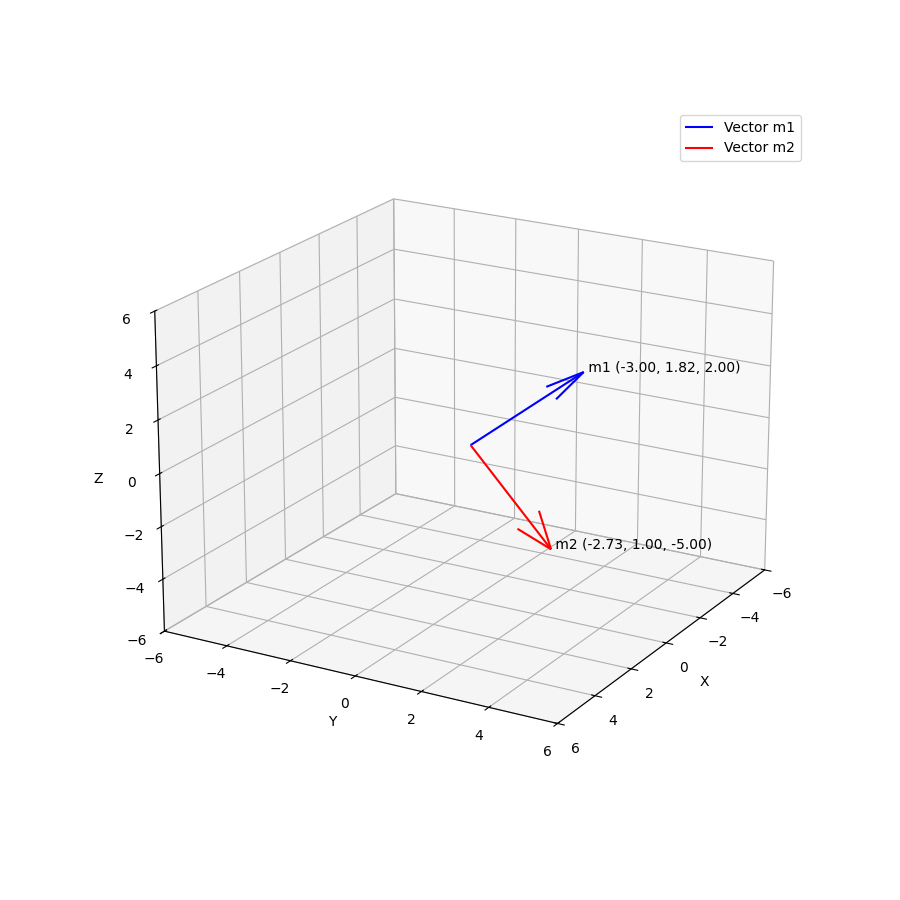
\includegraphics[width=0.8\linewidth]{figs/fig1.png}
	\caption{}
   \label{stemplot}
\end{figure}
\end{frame}

\section{C Code}
\begin{frame}[fragile]
\frametitle{C Code for Finding $p$ value}
\begin{lstlisting}[language=C]
include <math.h>
#include <stdio.h>
#include <stdlib.h>

int main() {

    double p;
    double m1_p_coeffs[3] = {0.0, 2.0/7.0, 0.0};
    double m1_consts[3] = {-3.0, 0.0, 2.0};

    double m2_p_coeffs[3] = {-3.0/7.0, 0.0, 0.0};
    double m2_consts[3] = {0.0, 1.0, -5.0};
    
    // Calculate A (the total coefficient for 'p') from the dot product expansion.
    double p_coefficient = (m1_consts[0] * m2_p_coeffs[0]) + (m1_p_coeffs[0] * m2_consts[0]) +(m1_consts[1] * m2_p_coeffs[1]) + (m1_p_coeffs[1] * m2_consts[1]) + (m1_consts[2] * m2_p_coeffs[2]) + (m1_p_coeffs[2] * 
    \end{lstlisting}
\end{frame}
\begin{frame}[fragile]
\frametitle{C Code for Finding $p$ value}
\begin{lstlisting}[language=C]
  m2_consts[2]);
// Calculate B (the total constant term) from the dot product expansion.
    double constant_term = (m1_consts[0] * m2_consts[0]) +
                         (m1_consts[1] * m2_consts[1]) +
                         (m1_consts[2] * m2_consts[2]);


    p = -constant_term / p_coefficient;

    double m1_final[3];
    double m2_final[3];

    m1_final[0] = m1_consts[0] + m1_p_coeffs[0] * p;
    m1_final[1] = m1_consts[1] + m1_p_coeffs[1] * p;
\end{lstlisting}
\end{frame}

\begin{frame}[fragile]
\frametitle{C Code for Finding $p$ value}
\begin{lstlisting}[language=C]
     m1_final[2] = m1_consts[2] + m1_p_coeffs[2] * p;
    m2_final[0] = m2_consts[0] + m2_p_coeffs[0] * p;
    m2_final[1] = m2_consts[1] + m2_p_coeffs[1] * p;
    m2_final[2] = m2_consts[2] + m2_p_coeffs[2] * p;


    FILE *file = fopen("values.dat", "w");
    if (file == NULL) {
        printf("Error opening file!\n");
        return 1;
    }

\end{lstlisting}
\end{frame}

\begin{frame}[fragile]
\frametitle{C Code for Finding $p$ value}
\begin{lstlisting}[language=C]
    fprintf(file, "%.4f %.4f %.4f\n", m1_final[0], m1_final[1], m1_final[2]);
    fprintf(file, "%.4f %.4f %.4f\n", m2_final[0], m2_final[1], m2_final[2]);

    fclose(file);
    printf("Direction vectors calculated and written to values.dat\n");
    printf("(The calculated value of p was: %.4f)\n", p);

    return 0;
}
\end{lstlisting}
\end{frame}

\section{Python Code}
\begin{frame}[fragile]
\frametitle{Python Code for Plotting}
\begin{lstlisting}[language=Python]
# Code by /sdcard/github/matgeo/codes/CoordGeoVV Sharma
# September 12, 2023
# Revised July 21, 2024
# Released under GNU GPL
# Section Formula

import sys
sys.path.insert(0, '/workspaces/urban-potato/matgeo/codes/CoordGeo/')  # path to my scripts
import numpy as np
import matplotlib.pyplot as plt
import matplotlib.image as mpimg
# Local imports
from line.funcs import *
from triangle.funcs import *
from conics.funcs import circ_gen

\end{lstlisting}
\end{frame}

\begin{frame}[fragile]
\frametitle{Python Code for Plotting}
\begin{lstlisting}[language=Python]
# Read data
data = np.loadtxt("values.dat", skiprows=1)

xc = data[0]  # Extract x-coordinate (e.g., -1)
yc = data[1]  # Extract y-coordinate (e.g., 4.5)

# Given points
A = np.array([-6, 7]).reshape(-1, 1)
B = np.array([-1, -5]).reshape(-1, 1)
P = np.array([xc, yc]).reshape(-1, 1)

# Generating line AB
x_AB = line_gen(A, B)

# Plotting
plt.plot(x_AB[0, :], x_AB[1, :], label='$AB$')

\end{lstlisting}
\end{frame}

\begin{frame}[fragile]
\frametitle{Python Code for Plotting}
\begin{lstlisting}[language=Python]
# Labeling the coordinates
tri_coords = np.block([[A, B, P]])
plt.scatter(tri_coords[0, :], tri_coords[1, :])

vert_labels = ['A', 'B', 'P']

# Helper function: format number with decimal only if needed
def fmt(val):
    return f"{val:.1f}" if abs(val - round(val)) > 1e-6 else f"{int(val)}"

for i, txt in enumerate(vert_labels):
    x = tri_coords[0, i].item()
    y = tri_coords[1, i].item()
    plt.annotate(f'{txt}\n({fmt(x)}, {fmt(y)})',
                 (x, y),
                 textcoords="offset points",
                 xytext=(20, -10),
                 ha='center')
\end{lstlisting}
\end{frame}

\begin{frame}[fragile]
\frametitle{Python Code for Plotting}
\begin{lstlisting}[language=Python]
ax = plt.gca()
ax.spines['left'].set_visible(False)
ax.spines['right'].set_visible(False)
ax.spines['top'].set_visible(False)
ax.spines['bottom'].set_visible(False)

plt.legend(loc='best')
plt.grid()

# Increase y-axis from -8 to 8 to show full range
plt.ylim(-7, 8)
plt.xlim(-7,7)

# Save and open
plt.show()
plt.savefig('../figs/fig1.png')
\end{lstlisting}
\end{frame}

\end{document}
